\documentclass[a4paper,11pt]{article}
\usepackage[english]{babel}
\usepackage[utf8]{inputenc}
\usepackage{graphicx}
\usepackage{float}
\usepackage{hyperref}
\usepackage{setspace}
\usepackage[left=2.5cm,right=2.5cm,top=2.5cm,bottom=2.5cm]{geometry}
\usepackage{pgfplots}
\pgfplotsset{compat=1.17}
\usepackage{amsmath}
\usepackage{amssymb}

\usepackage[automark,headsepline]{scrlayer-scrpage}
\pagestyle{scrheadings}
\ihead[]{Internet of Things (IIoT) and Manufacturing Execution Systems}
\ohead[]{Dmitrii Kochetov}
\cfoot[]{\pagemark}

\setlength{\parskip}{0.8em}
\setlength{\parindent}{0pt}

\usepackage{tikz}
\usetikzlibrary{shapes,arrows,positioning,calc}

\tikzstyle{block} = [draw, fill=white, rectangle, minimum height=3em, minimum width=4em]
\tikzstyle{sum} = [draw, fill=white, circle, node distance=1cm]
\tikzstyle{input} = [coordinate]
\tikzstyle{output} = [coordinate]
\tikzstyle{point} = [coordinate]

% PLC entity name macros — type names
\newcommand{\tyMotorState}{\texttt{MotorState}}
\newcommand{\tyMotorControl}{\texttt{MotorControl}}
\newcommand{\tyMotorControls}{\texttt{MotorControls}}
% PLC hardware
\newcommand{\cpuModel}{S7~1511-1~PN}
% PLC function and data block names
\newcommand{\fcRobot}{\texttt{FC\_Robot}}
\newcommand{\dbRobot}{\texttt{DB\_Robot}}
\newcommand{\fcControlMotor}{\texttt{Control/FC\_Control\_Motor}}
\newcommand{\fcSimMotor}{\texttt{Simulation/FC\_Simulation\_Motor}}
\newcommand{\fcUtilsRand}{\texttt{Utils/FC\_Utils\_Rand}}
\newcommand{\fcUtilsScale}{\texttt{Utils/FC\_Utils\_Scale}}
\newcommand{\fcUtilsWrap}{\texttt{Utils/FC\_Utils\_Wrap}}
% MotorState field names
\newcommand{\fEnable}{\texttt{Enable}}
\newcommand{\fSpeed}{\texttt{Speed}}
\newcommand{\fPosition}{\texttt{Position}}
\newcommand{\fTemperature}{\texttt{Temperature}}
\newcommand{\fPWM}{\texttt{PWM}}
\newcommand{\fRunning}{\texttt{Running}}
\newcommand{\fFault}{\texttt{Fault}}
% MotorControl field names
\newcommand{\fTargetSpeed}{\texttt{TargetSpeed}}
\newcommand{\fOverridePWM}{\texttt{OverridePWM}}
\newcommand{\fEnableOverridePWM}{\texttt{EnableOverridePWM}}
\newcommand{\fStop}{\texttt{Stop}}
\newcommand{\fKp}{\texttt{Kp}}

\begin{document}

\tableofcontents
\newpage

\section{Introduction}

This project aims to develop a PLC-connected HMI system as part of the lecture ``IoT \& MES''.
The goal is to design a modular architecture that enables monitoring and control of a simulated
system using modern tools and technologies, reflecting the Industrie~4.0 vision of interconnected,
data-driven production systems.

The implemented system simulates a robotic vehicle with two independently controlled motors representing
the left and right wheels. Instead of implementing complex motion logic directly on the PLC, the system
separates responsibilities across different components.

A Python-based backend is used as an intermediary layer between the PLC, database, and dashboard.
This design allows flexible data processing and avoids reliance on visual programming tools such as
Node-RED. The overall system emphasizes modularity, decoupling, and reproducibility through containerization.

A further goal is to follow the \textit{Infrastructure as Code} (IaC) principle, meaning that all
infrastructure components---containers, service configurations, and environment definitions---are
fully described in declarative configuration files. Version control plays a central role in achieving
this, as it ensures traceability of changes, supports collaboration, and allows the entire system
state to be restored or replicated at any point in time.

\section{System Overview}

\subsection{Architecture}

The system consists of the following main components:

% TODO: add references to the corresponding sections describing each component in more detail
\begin{itemize}
    \item PLC simulated using TIA Portal and PLCSIM
    \item Python backend acting as communication layer
    \item InfluxDB as time-series database
    \item Grafana for visualization and user interaction
    \item Docker for containerized deployment (except PLC)
\end{itemize}

The PLC is responsible for simulating the machine behavior, while Python handles communication and
data processing. The database and dashboard are fully decoupled from the PLC.
The overall structure is illustrated in \autoref{fig:architecture}.

\begin{figure}[H]
    \centering
    \includegraphics[width=\textwidth]{.export/architecture-Architecture}
    \caption{System Architecture}
    \label{fig:architecture}
\end{figure}

\subsection{Data Flow}

The system follows a clearly defined data flow:

\begin{itemize}
    \item The PLC exposes process variables via OPC UA and accepts setpoint values written to its
    OPC UA nodes
    \item Python subscribes to OPC UA value changes and additionally polls the PLC periodically for
    snapshots, storing the results in InfluxDB
    \item Grafana retrieves data from InfluxDB for visualization
    \item User interactions in Grafana are sent to Python
    \item Python processes the requests, stores them in InfluxDB, and writes the corresponding
    values back to the PLC
\end{itemize}

\section{PLC Implementation}

\subsection{Hardware Selection}

The simulated PLC is a Siemens \cpuModel{}. For a real deployment a CPU from the S7-1200 series
would be sufficient for this application; however, the \cpuModel{} was chosen due to a tooling
constraint: PLCSIM Advanced is required to simulate an OPC UA server, and it does not support the
1200 series. Within the 1500 series the \cpuModel{} is the entry-level model, so it was the
natural choice.

\subsection{Program Structure}

The PLC project is structured into a main OB, a robot function block, per-motor control and
simulation function blocks, a global data block, and a set of utility functions.
The main OB simply calls \fcRobot{}, which iterates over the \tyMotorControls{} array and invokes
\fcControlMotor{} and \fcSimMotor{} for each entry in sequence.
All motor state and setpoints are stored persistently in \dbRobot{}, which holds the
\tyMotorControls{} array described in the next section.

\subsection{Data Structures}
\label{sec:plc-data-structures}

The PLC program uses two custom structured data types and an array to represent the system state and
control interface.

\textbf{\tyMotorState} captures the current status of a single motor and is exposed as read-only via
OPC UA:

\begin{itemize}
    \item \fEnable{} (Bool) --- whether the motor is enabled
    \item \fSpeed{} (Real) --- current rotational speed in deg/s
    \item \fPosition{} (Real) --- accumulated angular position in degrees (0--360)
    \item \fTemperature{} (Real) --- motor temperature in \textdegree{}C
    \item \fPWM{} (Real) --- current PWM duty cycle (0.0 = full reverse, 1.0 = full forward)
    \item \fRunning{} (Bool) --- indicates active motor operation
    \item \fFault{} (Bool) --- fault flag
\end{itemize}

\textbf{\tyMotorControl} groups all writable setpoints together with the embedded read-only state for
a single motor:

\begin{itemize}
    \item \fTargetSpeed{} (Real) --- desired rotational speed setpoint in deg/s (read/write)
    \item \fOverridePWM{} (Real) --- manual PWM override value (0.0 = full reverse, 1.0 = full forward; read/write)
    \item \fEnableOverridePWM{} (Bool) --- activates the PWM override mode (read/write)
    \item \fStop{} (Bool) --- issues a stop command to the motor (read/write)
    \item \fKp{} (Real) --- proportional gain for the speed controller (read/write)
    \item \tyMotorState{} --- nested field of type \tyMotorState{} (read-only)
\end{itemize}

\textbf{\tyMotorControls} is an array of two \tyMotorControl{} instances. This array is the
top-level OPC UA object through which external components access both motors uniformly.

This design covers the requirement of using different data structures: a struct for grouping related
fields, nesting to embed state inside a control block, and an array to hold multiple motors. A key
benefit is that the PLC itself is not aware of which motor is ``left'' or ``right''---it simply
operates on array indices. The interpretation is left to higher-level components. Adding a third
motor would only require extending the array, with no changes to the data types themselves.

\subsection{Simulation Model}

\fcSimMotor{} models each motor per PLC cycle: \fPWM{} is clamped and mapped to a target speed,
which the actual speed tracks with a first-order lag and random jitter. Position is integrated from
speed and wrapped to 0--360\textdegree{}. Temperature follows speed via a quadratic target and a
thermal lag. \fRunning{} stays set while the motor is enabled, still coasting, or still warm.

Three utility functions support the model: \fcUtilsRand{} (random jitter),
\fcUtilsScale{} (range mapping), and \fcUtilsWrap{} (angle wrapping).

\subsection{Control Logic}

\fcControlMotor{} runs a simple P-controller each cycle with \fTargetSpeed{} as the setpoint and
\fPWM{} as the output. Setting \fEnableOverridePWM{}
bypasses the controller and writes \fOverridePWM{} directly; \fStop{} disables the motor
immediately. Higher-level kinematics are handled outside the PLC.

\section{Communication Interface}

\subsection{Python Backend}

The Python backend is the central communication layer of the system, connecting to the PLC via
OPC UA, translating user commands from the dashboard into PLC setpoints, storing process data in
InfluxDB, and performing kinematic calculations to convert high-level motion parameters (linear and
angular velocity) into individual wheel speed setpoints.

\subsection{Architectural Decisions}

\subsubsection{Choice of Python over Node-RED}

The project brief suggested Node-RED as one possible integration tool. Python was chosen instead
for the following reasons:

\begin{itemize}
    \item \textbf{Execution flow control} --- Python allows fine-grained control over asynchronous
    tasks, error handling, and retry logic. Node-RED's visual wiring model makes such orchestration
    harder to reason about and maintain.
    \item \textbf{Version control} --- plain Python source files integrate naturally with Git,
    making every change fully traceable and reviewable. Node-RED flows are stored as JSON, which is
    difficult to review meaningfully in a diff.
    \item \textbf{Personal preference} --- from a personal perspective, Python feels more
    professional and appropriate for a backend service than a visual flow editor primarily aimed
    at rapid prototyping.
\end{itemize}

\subsubsection{OPC UA over a S7-specific library}

An alternative would have been to use a Siemens-specific library (e.g.\ snap7 via python-snap7)
to communicate directly with the S7 PLC. OPC UA was chosen instead for the following reasons:

\begin{itemize}
    \item \textbf{Manufacturer independence} --- any device exposing an OPC UA server can be
    integrated without modifying the backend, decoupling it from Siemens-specific protocol details.
    \item \textbf{Standardization} --- OPC UA is an open, platform-independent IEC standard widely
    adopted in industrial automation.
    \item \textbf{Explicit access control} --- the PLC declares which nodes are readable and
    writable in its address space; the backend respects those declarations rather than relying on
    undocumented memory mappings.
\end{itemize}

\subsection{Backend Architecture}
\label{sec:backend-architecture-text}

The internal structure of the Python backend is illustrated in \autoref{fig:backend-architecture}.

\begin{figure}[H]
    \centering
    \includegraphics[width=\textwidth]{.export/backend-architecture-Backend-Architecture}
    \caption{Python Backend Architecture}
    \label{fig:backend-architecture}
\end{figure}

The backend is organized into four layers: the \textbf{API layer} exposes HTTP endpoints for
Grafana commands, the \textbf{domain layer} contains business logic and kinematic conversion, the
\textbf{infrastructure layer} provides OPC UA and InfluxDB adapters, and the
\textbf{application layer} routes commands and data between them. In the OPC UA adapter,
subscriptions are the primary path for low-latency updates without unnecessary reads, while slower
polling (about 15--30\,s) is used as a practical workaround to keep Grafana fed during quiet
periods; in real systems, the same mechanism can also serve periodic snapshot requirements. In the
database path, the backend also persists \texttt{motion\_intent} (which does not exist on the PLC)
and periodically rewrites the latest value as another explicit workaround to avoid empty or
discontinuous Grafana panels after restarts or long inactive phases.

\section{Data Storage}

\subsection{Database Choice}

InfluxDB~2 was selected because the project primarily handles time-stamped process signals and
control intents. It integrates directly with Grafana through Flux queries and is a natural fit for
continuous telemetry from the PLC. It is also a widely adopted, modern, and well-established
industry tool for time-series workloads, so using it in this project is valuable from a learning
perspective.

\subsection{Storage Responsibilities}

The database layer has two core responsibilities: persisting telemetry from the PLC-facing OPC UA
path and persisting high-level control intent from the API path. This keeps observability data and
operator intent in one time-aligned history, which simplifies analysis and dashboard queries.

\subsection{Data Model}

The backend writes two main measurement groups to the robot bucket:

\begin{itemize}
    \item \textbf{Wheel telemetry and configuration} from OPC UA samples
    (e.g. speed, temperature, PWM, target speed, controller parameters; see
    \autoref{sec:plc-data-structures}), tagged by
    \texttt{wheel\_side}
    \item \textbf{Motion intent} (\texttt{v}, \texttt{omega}, \texttt{emergency\_stop}), which is an
    application-level command history and does not exist as a native PLC signal (see
    \autoref{sec:backend-architecture-text})
\end{itemize}

InfluxDB assigns timestamps to all points, enabling historical analysis and continuous visualization
in Grafana.

\section{Dashboard}

\subsection{Choice of Grafana}

Grafana was chosen as the dashboard implementation for the following reasons:

\begin{itemize}
    \item \textbf{Professional data visualization} --- Grafana is a widely adopted, production-grade
    observability platform with a rich set of panel types, flexible query editors, and multi-series
    layouts out of the box.
    \item \textbf{Personal preference} --- although not the most common choice for machine-level
    HMIs, Grafana is well established in the IT and DevOps world. It is relatively easy to
    configure and produces polished dashboards with minimal effort, making it a good tool to learn.
\end{itemize}

\subsection{Grafana Setup}

Grafana serves as the visualization and control front-end of the system. Its InfluxDB datasource
and default dashboard are provisioned automatically from configuration files at container startup,
so no manual Grafana setup is required after deployment. The datasource uses the Flux query
language and connects to InfluxDB. The default auto-refresh interval is set to one second, enabling
near real-time display of live process data. The operator can also freely adjust the time range to
analyze historical motor behavior: zooming in on a specific event, scrolling back in time, or
pausing live updates to inspect a captured interval.

\subsection{Visualization}

The dashboard is shown in \autoref{fig:hmi-screenshot} and is organized into three rows.

\begin{figure}[H]
    \centering
    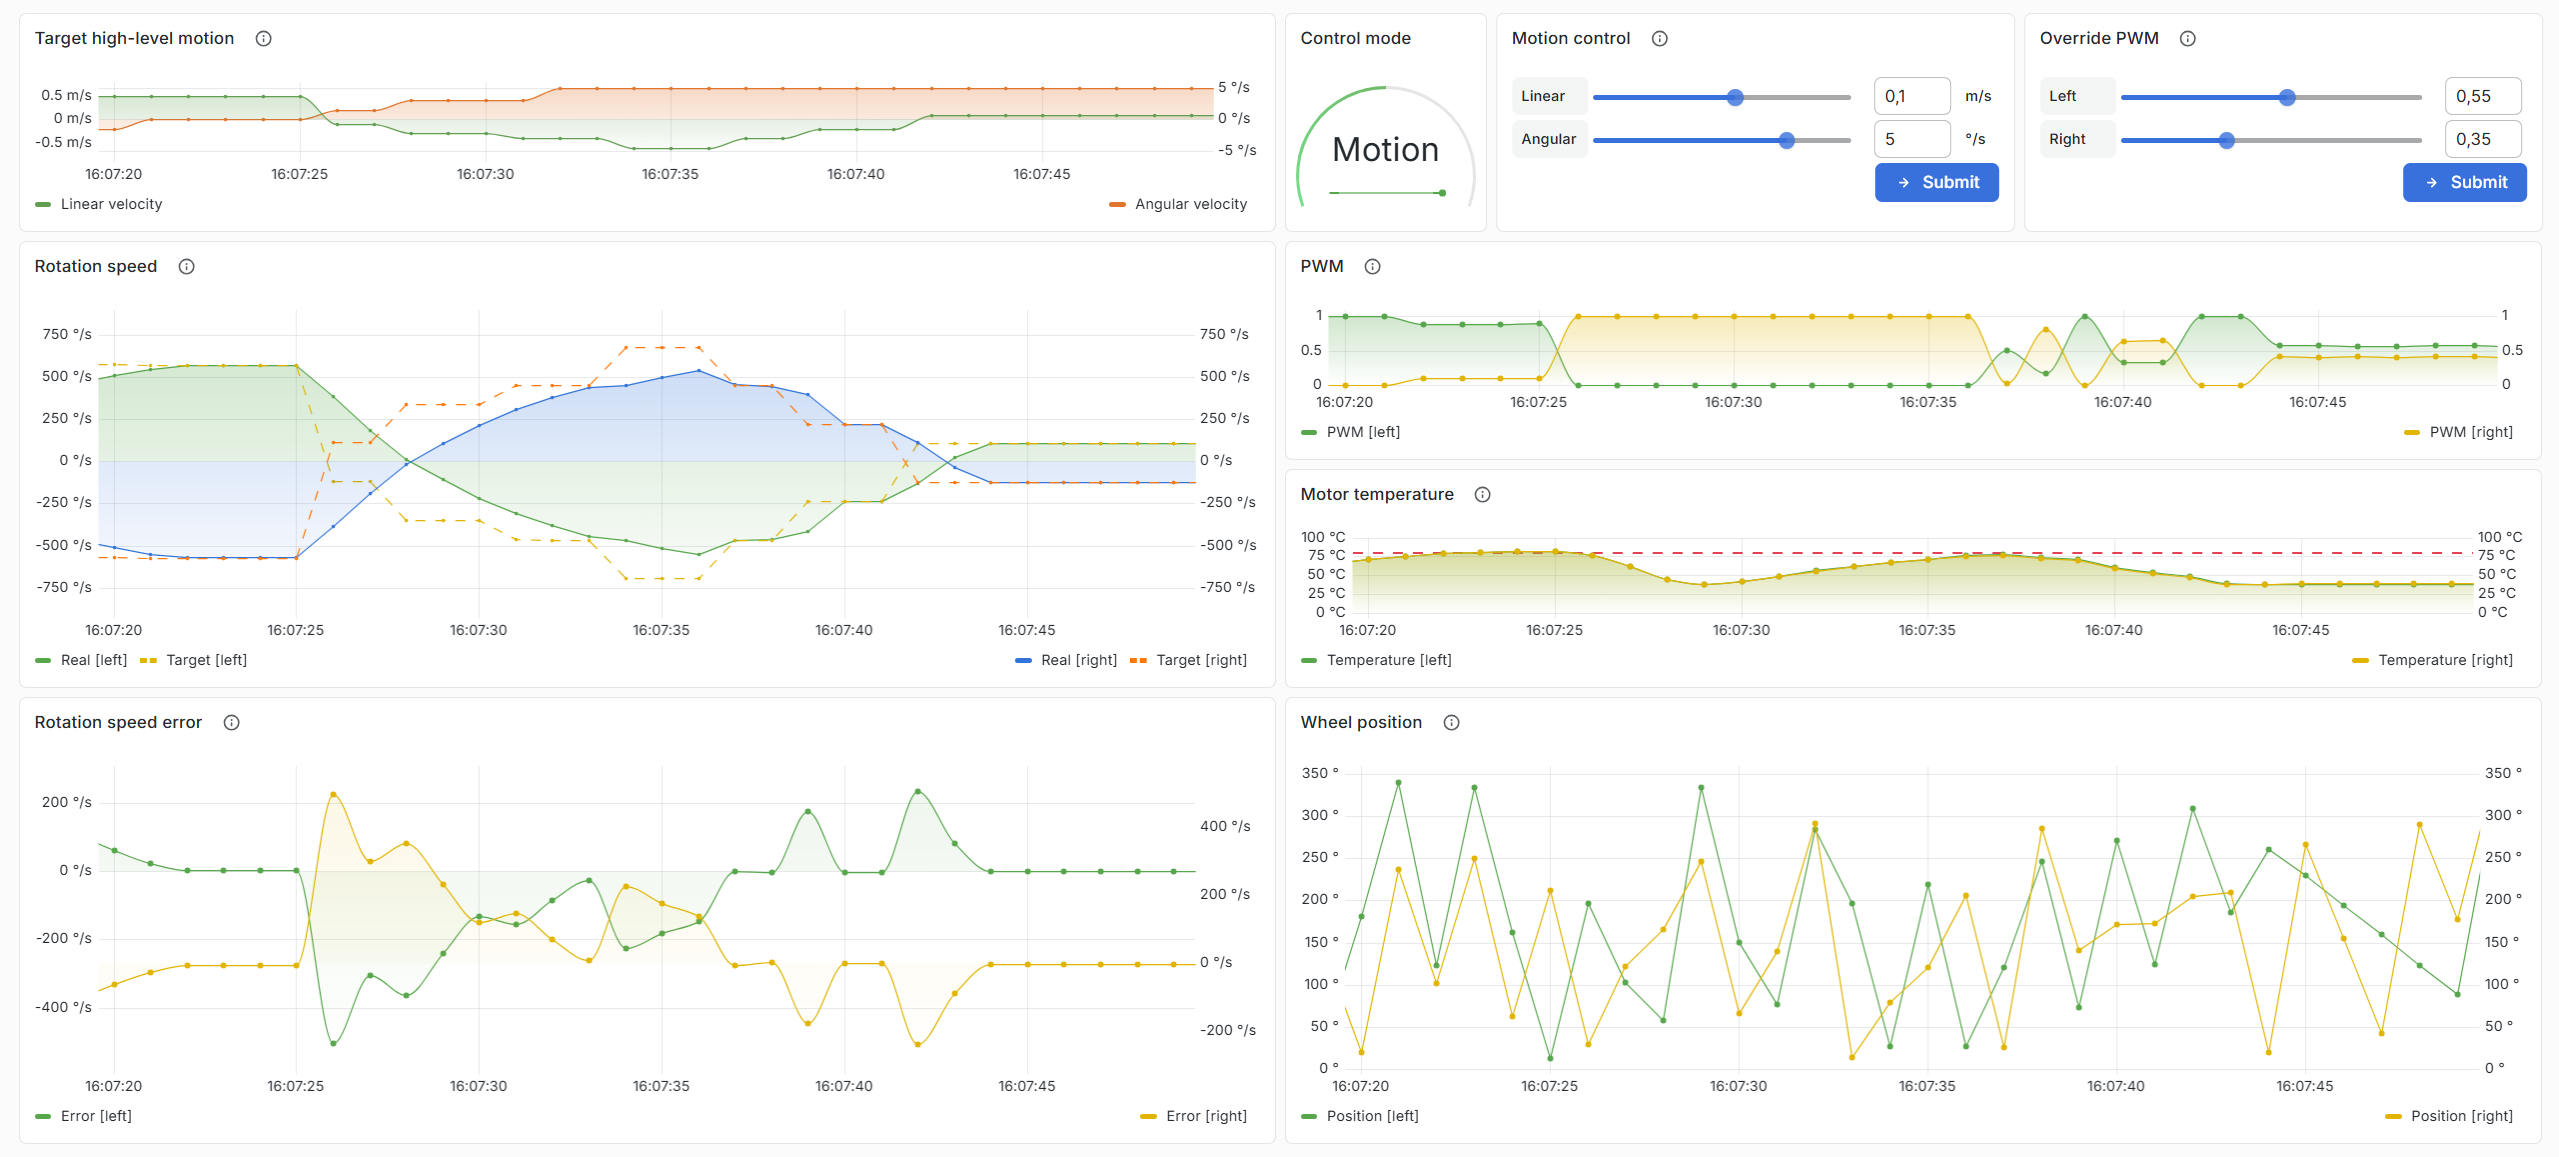
\includegraphics[width=\textwidth]{diagrams/hmi-screenshot}
    \caption{Grafana Dashboard}
    \label{fig:hmi-screenshot}
\end{figure}

The top row shows the high-level motion state alongside the two interactive control panels
described in \autoref{sec:dashboard-interaction}: a time-series chart of target linear and angular
velocity (\texttt{v} and \texttt{omega} from the \texttt{motion\_intent} measurement), an
indicator for the active control mode (Motion or PWM Override), and the two form-based input
panels.

The middle and lower rows contain five read-only monitoring plots, all sourcing from the
\texttt{wheel\_state} measurement tagged by \texttt{wheel\_side}:

\begin{itemize}
    \item \textbf{Rotation speed} --- actual and target speed (deg/s) for each wheel side;
    target speed is drawn as a dashed line to keep it visually distinct from the measured value
    \item \textbf{Rotation speed error} --- difference between target and actual speed, useful for
    assessing P-controller tracking performance
    \item \textbf{PWM} --- duty cycle (0.0 = full reverse, 1.0 = full forward) per wheel
    \item \textbf{Motor temperature} --- temperature in \textdegree{}C per wheel, with a threshold
    marker at 80\textdegree{}C to indicate thermal stress
    \item \textbf{Wheel position} --- accumulated angular position (0--360\textdegree{}) per wheel
\end{itemize}

\subsection{Interaction}
\label{sec:dashboard-interaction}

User interaction is implemented via the Volkov Labs Business Forms plugin, which renders slider
controls and submits their values as HTTP POST requests directly to the Python backend. Grafana
never communicates with the PLC.

Two independent control panels are provided, each corresponding to one of the two backend API
endpoints (see \autoref{sec:backend-architecture-text}):

\begin{itemize}
    \item \textbf{Motion control} --- sliders for linear velocity $v$
    ($-1$ to $1$\,m/s) and angular velocity $\omega$ ($-10$ to $10$\,\textdegree{}/s), submitted
    to \texttt{/command/motion}
    \item \textbf{Override PWM} --- independent left and right PWM sliders (0 to 1), submitted to
    \texttt{/command/pwm\_override}
\end{itemize}

The active control mode is reflected in the \emph{Control mode} gauge, which reads
\texttt{pwm\_override\_enable} from the stored telemetry and displays either ``Motion'' or ``PWM''.

\section{Deployment}

\subsection{Docker Architecture}

The following components are containerized:

\begin{itemize}
    \item Python backend
    \item InfluxDB
    \item Grafana
\end{itemize}

This simplifies deployment and ensures consistent environments.

\subsection{Setup Strategy}

Docker allows:

\begin{itemize}
    \item Easy setup
    \item Reproducibility
    \item Isolation of components
\end{itemize}

All services can be started using a single configuration.

\subsection{VM and Host Setup}

The PLC environment (TIA Portal and PLCSIM) runs inside a virtual machine, while Docker containers
run on the host system.

This setup separates engineering tools from runtime services.

\subsection{Alternative Deployment Strategies}

Different deployment strategies were evaluated:

\begin{itemize}
    \item Running all components on the host system
    \item Running all components inside a virtual machine
\end{itemize}

Each approach has trade-offs regarding networking, performance, and complexity. The chosen hybrid
setup provides a good balance between usability and stability.

\section{Setup Guide}

To run the system:

\begin{enumerate}
    \item Open the TIA Portal project
    \item Start PLCSIM and load the PLC program
    \item Start the Docker containers
    \item Run the Python backend
    \item Open Grafana in a web browser
\end{enumerate}

After these steps, the system should be fully operational.

\section{Results and Discussion}

The system successfully demonstrates a working PLC-connected dashboard:

\begin{itemize}
    \item Reliable data exchange between components
    \item Clear separation of responsibilities
    \item Functional visualization and control
\end{itemize}

Limitations include the use of simulation instead of real hardware and potential latency introduced
by multiple system layers.

\section{Conclusion}

The project achieves its goal of building a modular PLC-connected dashboard system. The architecture
allows flexible interaction between industrial and modern software components.

Future improvements could include integration of real hardware, more advanced simulations, or
additional control algorithms.

\appendix
\section{Appendix}
Additional materials such as screenshots, variable lists, or configuration files can be included here.

\end{document}